% Options for packages loaded elsewhere
\PassOptionsToPackage{unicode}{hyperref}
\PassOptionsToPackage{hyphens}{url}
%
\documentclass[
]{article}
\usepackage{lmodern}
\usepackage{amssymb,amsmath}
\usepackage{ifxetex,ifluatex}
\ifnum 0\ifxetex 1\fi\ifluatex 1\fi=0 % if pdftex
  \usepackage[T1]{fontenc}
  \usepackage[utf8]{inputenc}
  \usepackage{textcomp} % provide euro and other symbols
\else % if luatex or xetex
  \usepackage{unicode-math}
  \defaultfontfeatures{Scale=MatchLowercase}
  \defaultfontfeatures[\rmfamily]{Ligatures=TeX,Scale=1}
\fi
% Use upquote if available, for straight quotes in verbatim environments
\IfFileExists{upquote.sty}{\usepackage{upquote}}{}
\IfFileExists{microtype.sty}{% use microtype if available
  \usepackage[]{microtype}
  \UseMicrotypeSet[protrusion]{basicmath} % disable protrusion for tt fonts
}{}
\makeatletter
\@ifundefined{KOMAClassName}{% if non-KOMA class
  \IfFileExists{parskip.sty}{%
    \usepackage{parskip}
  }{% else
    \setlength{\parindent}{0pt}
    \setlength{\parskip}{6pt plus 2pt minus 1pt}}
}{% if KOMA class
  \KOMAoptions{parskip=half}}
\makeatother
\usepackage{xcolor}
\IfFileExists{xurl.sty}{\usepackage{xurl}}{} % add URL line breaks if available
\IfFileExists{bookmark.sty}{\usepackage{bookmark}}{\usepackage{hyperref}}
\hypersetup{
  pdftitle={User Guide - Understanding Airbnb listings in Australia},
  hidelinks,
  pdfcreator={LaTeX via pandoc}}
\urlstyle{same} % disable monospaced font for URLs
\usepackage[margin=1in]{geometry}
\usepackage{graphicx,grffile}
\makeatletter
\def\maxwidth{\ifdim\Gin@nat@width>\linewidth\linewidth\else\Gin@nat@width\fi}
\def\maxheight{\ifdim\Gin@nat@height>\textheight\textheight\else\Gin@nat@height\fi}
\makeatother
% Scale images if necessary, so that they will not overflow the page
% margins by default, and it is still possible to overwrite the defaults
% using explicit options in \includegraphics[width, height, ...]{}
\setkeys{Gin}{width=\maxwidth,height=\maxheight,keepaspectratio}
% Set default figure placement to htbp
\makeatletter
\def\fps@figure{htbp}
\makeatother
\setlength{\emergencystretch}{3em} % prevent overfull lines
\providecommand{\tightlist}{%
  \setlength{\itemsep}{0pt}\setlength{\parskip}{0pt}}
\setcounter{secnumdepth}{-\maxdimen} % remove section numbering

\title{User Guide - Understanding Airbnb listings in Australia}
\author{true \and true \and true}
\date{}

\begin{document}
\maketitle

\hypertarget{exploratory-data-analysis-eda}{%
\section{Exploratory Data Analysis
(EDA)}\label{exploratory-data-analysis-eda}}

Exploratory Data Analysis allows you to perform initial investigation on
the data, so that you may be able to discover patterns, and explore the
different variables in the data set. It will allow us to formulate
hypothesis and explore different statistics models that could be
developed after.

\hypertarget{bar-charts}{%
\subsection{Bar Charts}\label{bar-charts}}

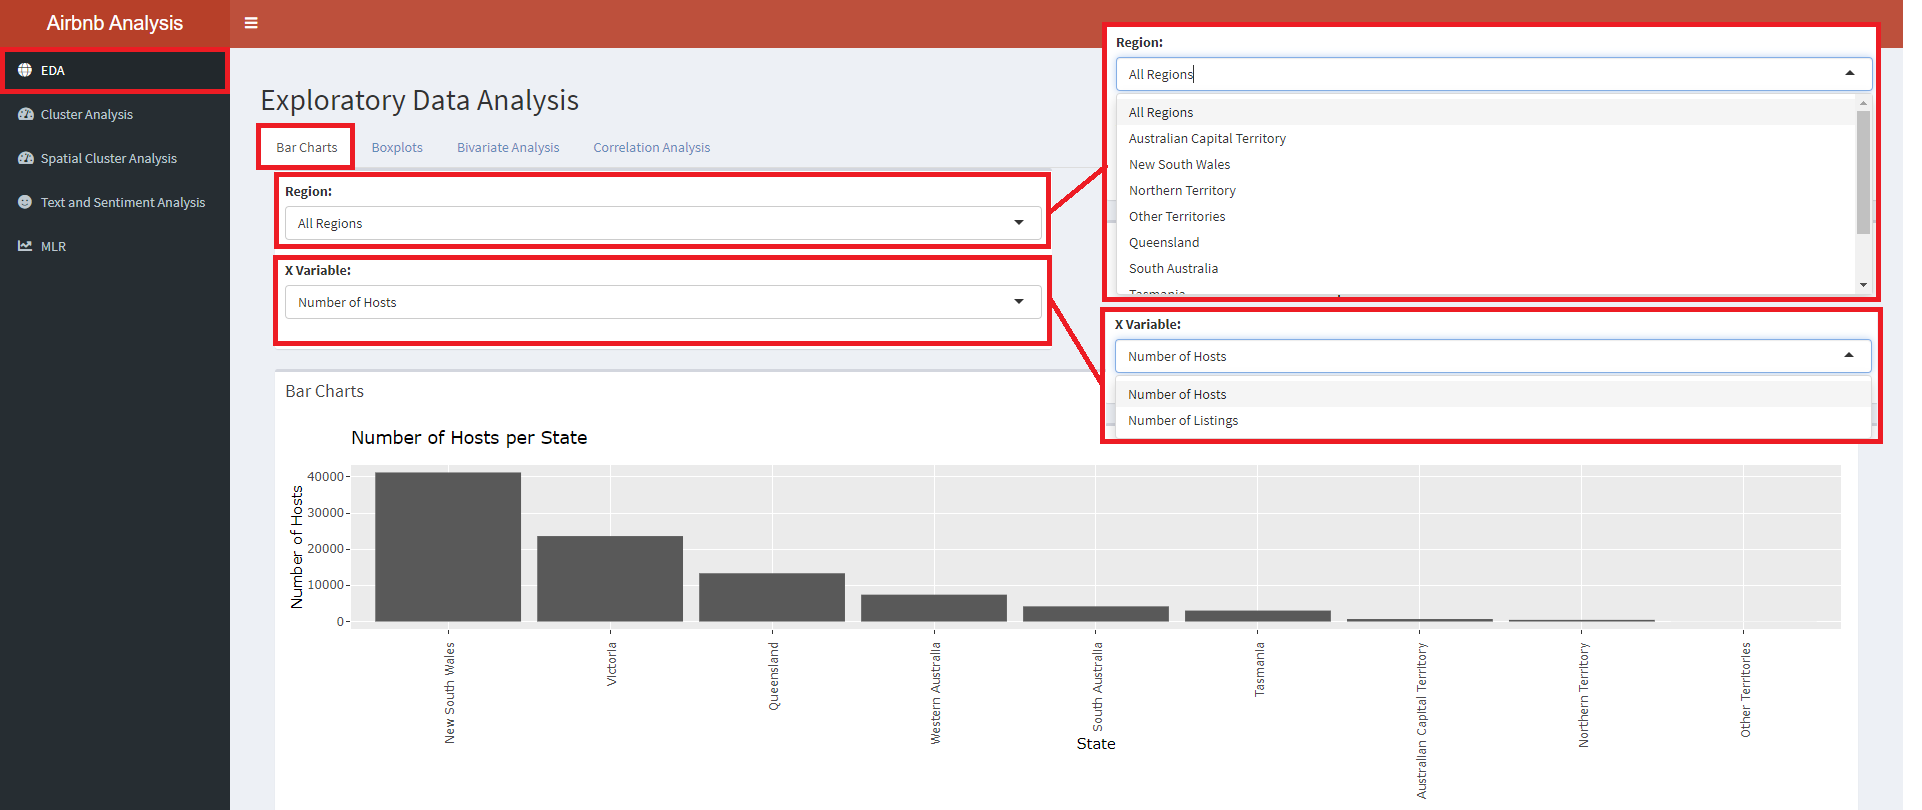
\includegraphics[width=0.6\textwidth,height=\textheight]{images/edabar.png}

\begin{itemize}
\tightlist
\item
  Click on \emph{``Region:''} to explore the different states in
  Australia
\item
  Click on \emph{``X Variable:''} to explore \emph{``Number of Hosts''}
  and \emph{``Number of Listings''} in various different States.
\end{itemize}

The top barchart showcases the \emph{``X Variable''} per State.

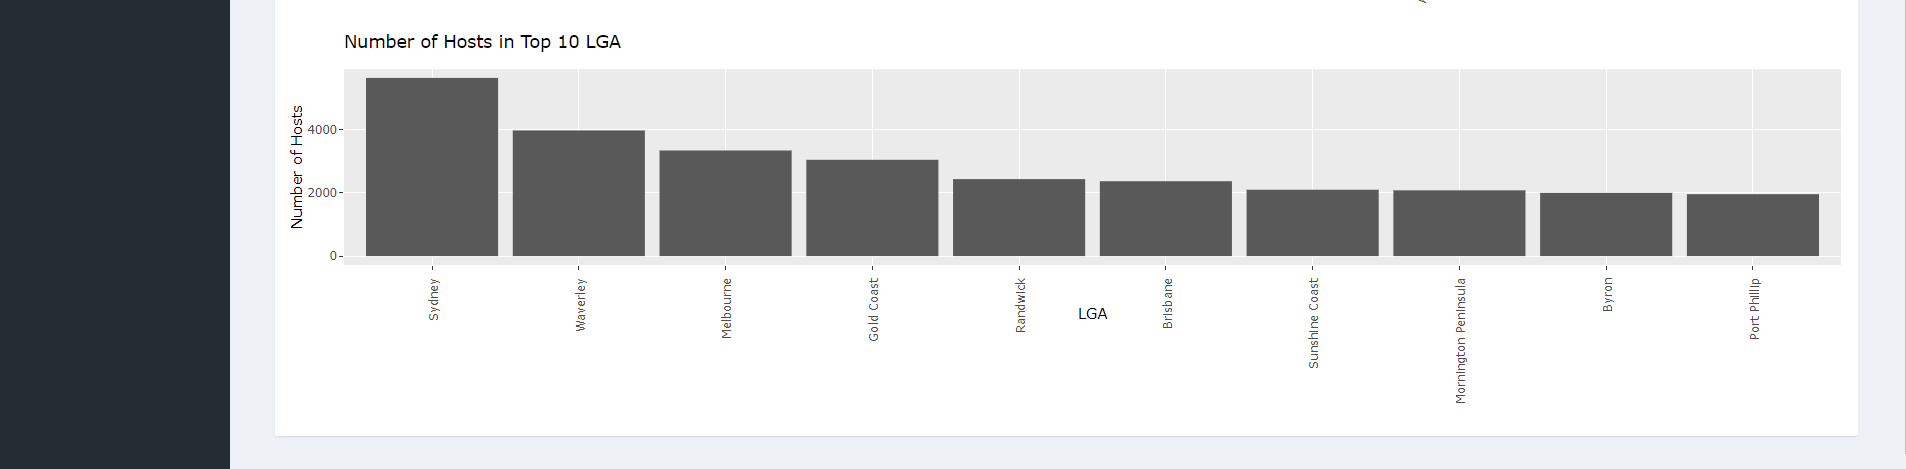
\includegraphics[width=0.6\textwidth,height=\textheight]{images/edabar2.png}

The bottom barchart showcases the \emph{``X Variable''} per top 10 Local
Government Area per State.

\hypertarget{boxplots}{%
\subsection{Boxplots}\label{boxplots}}

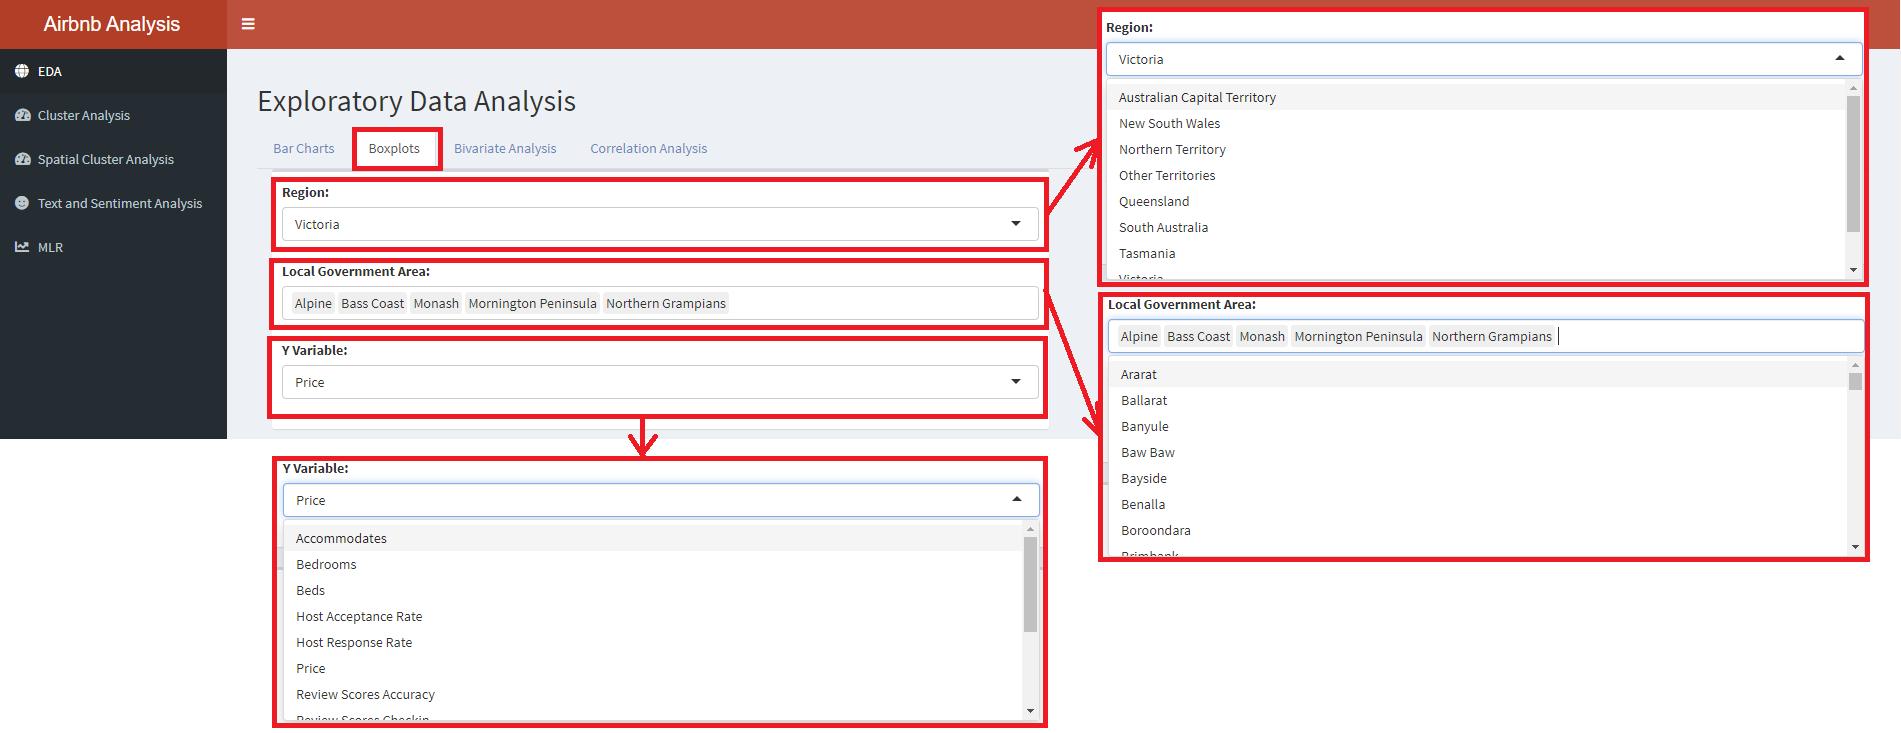
\includegraphics[width=0.6\textwidth,height=\textheight]{images/edabox.png}

\begin{itemize}
\tightlist
\item
  Click on \emph{``Region:''} to explore the different states in
  Australia.
\item
  Click on \emph{``Local Government Area''} to explore the different
  cities in the State. You are able to choose multiple cities to view at
  a single time through clicking the chosen city in the drop down bar.
\item
  Click on \emph{``Y Variable:''} to view the boxplots of different
  variables such as \emph{Price, Review Scores Ratings, Bedrooms, Beds}
  etc.
\end{itemize}

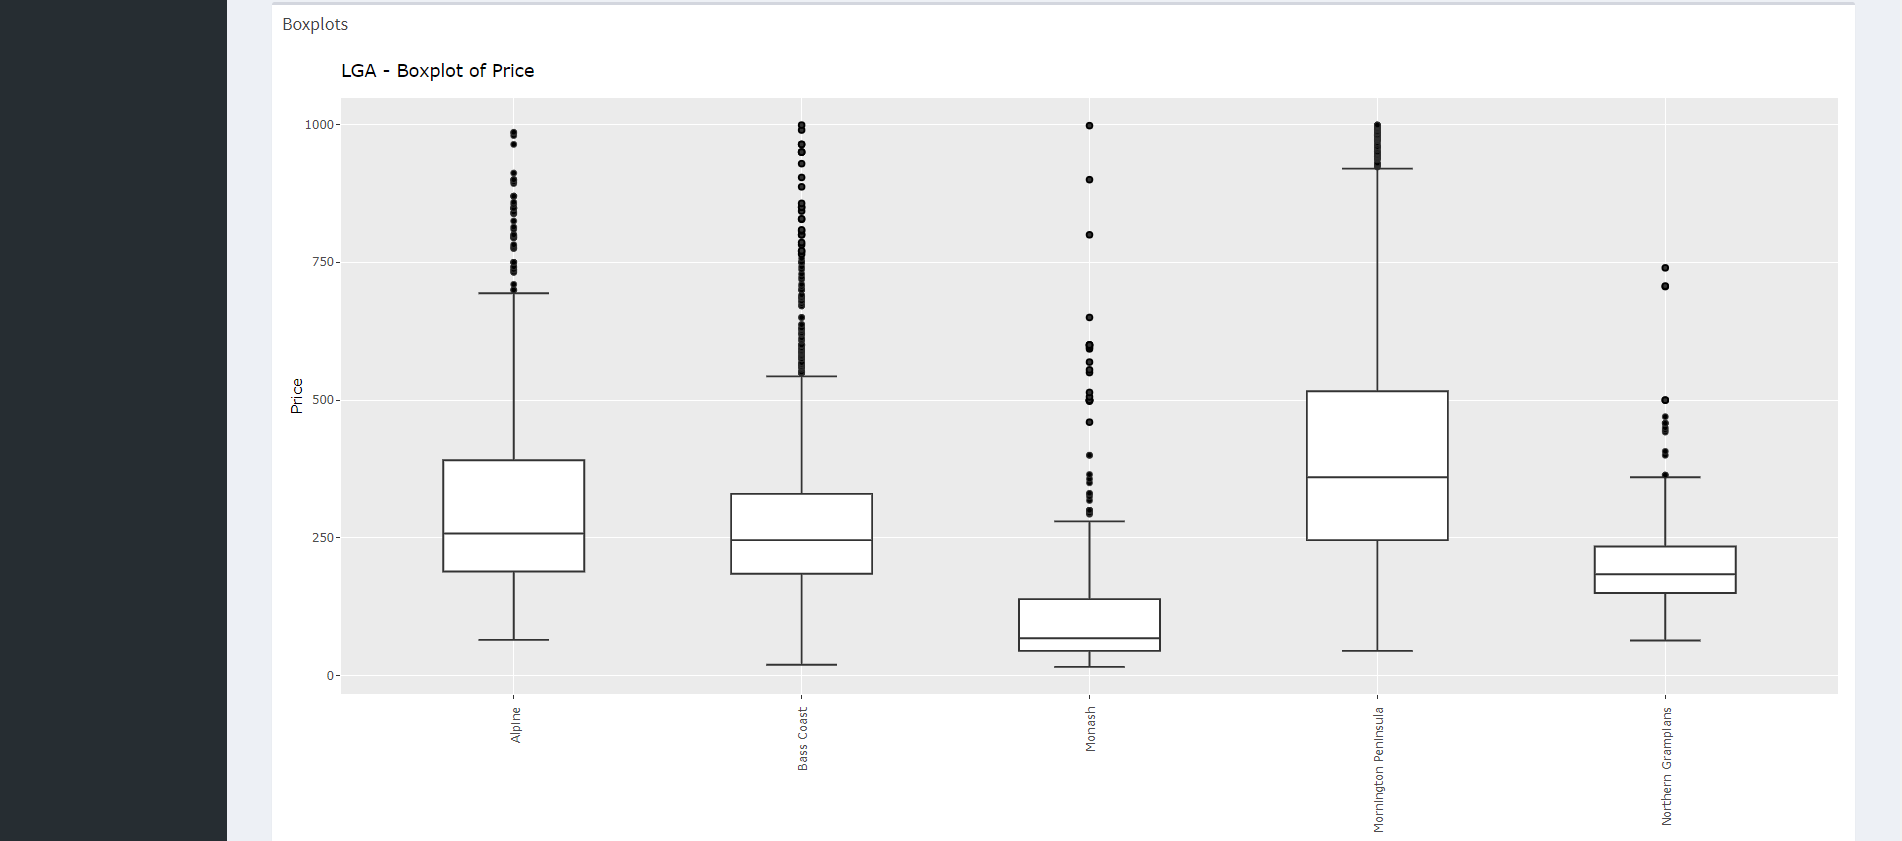
\includegraphics[width=0.6\textwidth,height=\textheight]{images/edabox2.png}

The top boxplot showcases Boxplots of \emph{``Y Variable''} against the
Local Government Area.

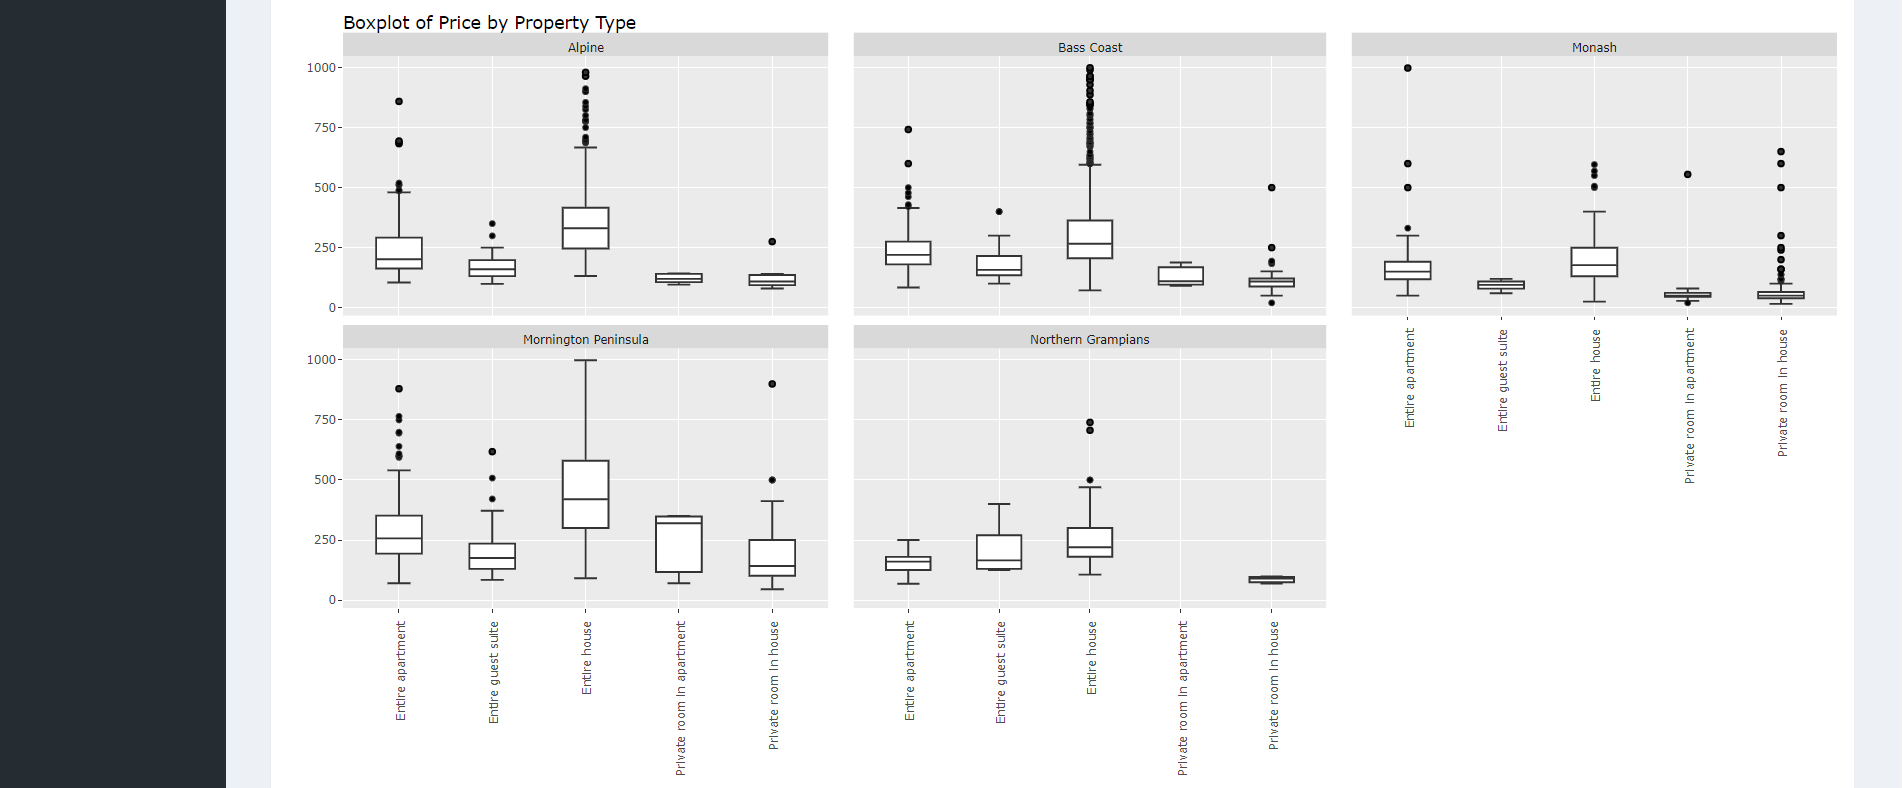
\includegraphics[width=0.6\textwidth,height=\textheight]{images/edabox3.png}

The bottom boxplot showcases \emph{``Price''} vs \emph{``Property
Type''} with a Facet Wrap of Local Government Area.

\hypertarget{bivariate-analysis}{%
\subsection{Bivariate Analysis}\label{bivariate-analysis}}

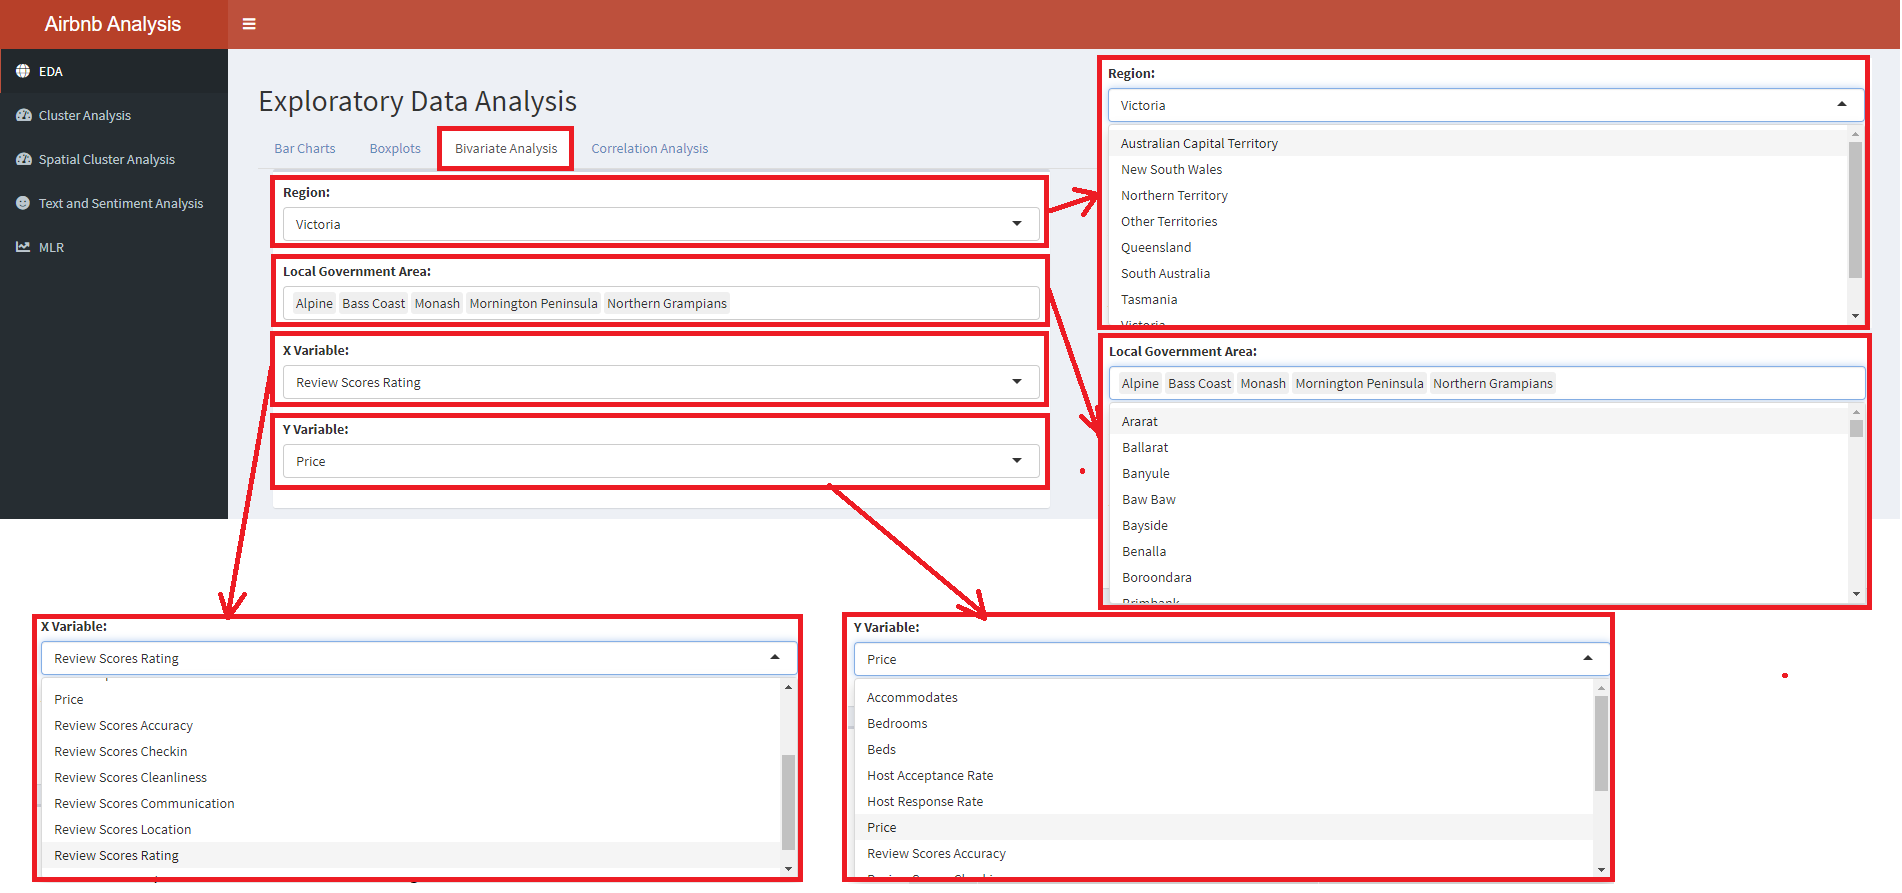
\includegraphics[width=0.6\textwidth,height=\textheight]{images/edabivariate.png}

\begin{itemize}
\tightlist
\item
  Click on \emph{``Region:''} to explore the different states in
  Australia.
\item
  Click on \emph{``Local Government Area''} to explore the different
  cities in the State. You are able to choose multiple cities to view at
  a single time through clicking the chosen city in the drop down bar.
\item
  Click on \emph{``X Variable:''} and \emph{``Y Variable:''} to view the
  bivariate plot with different variables such as \emph{Price, Review
  Scores Ratings, Bedrooms, Beds} etc. This will allow us to explore how
  2 variables interact with each other
\end{itemize}

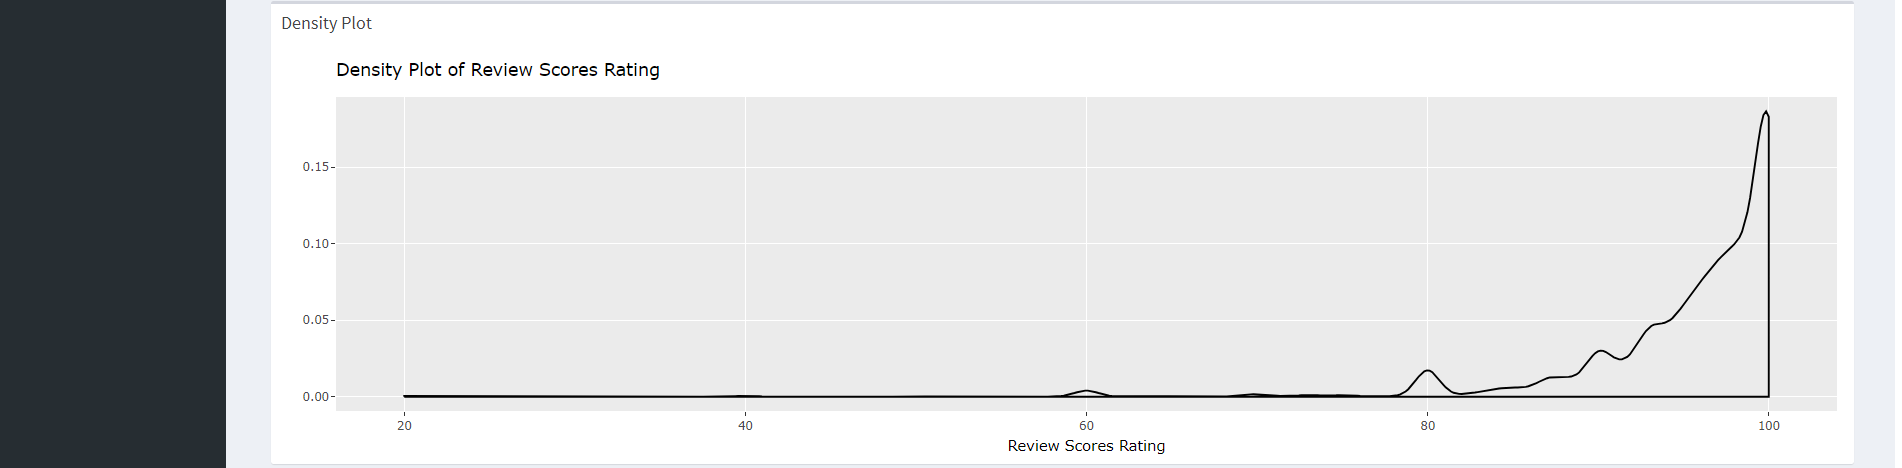
\includegraphics[width=0.6\textwidth,height=\textheight]{images/edabivariate2.png}

The top plot is a density plot to showcase the density of the \emph{``X
Variable''}.

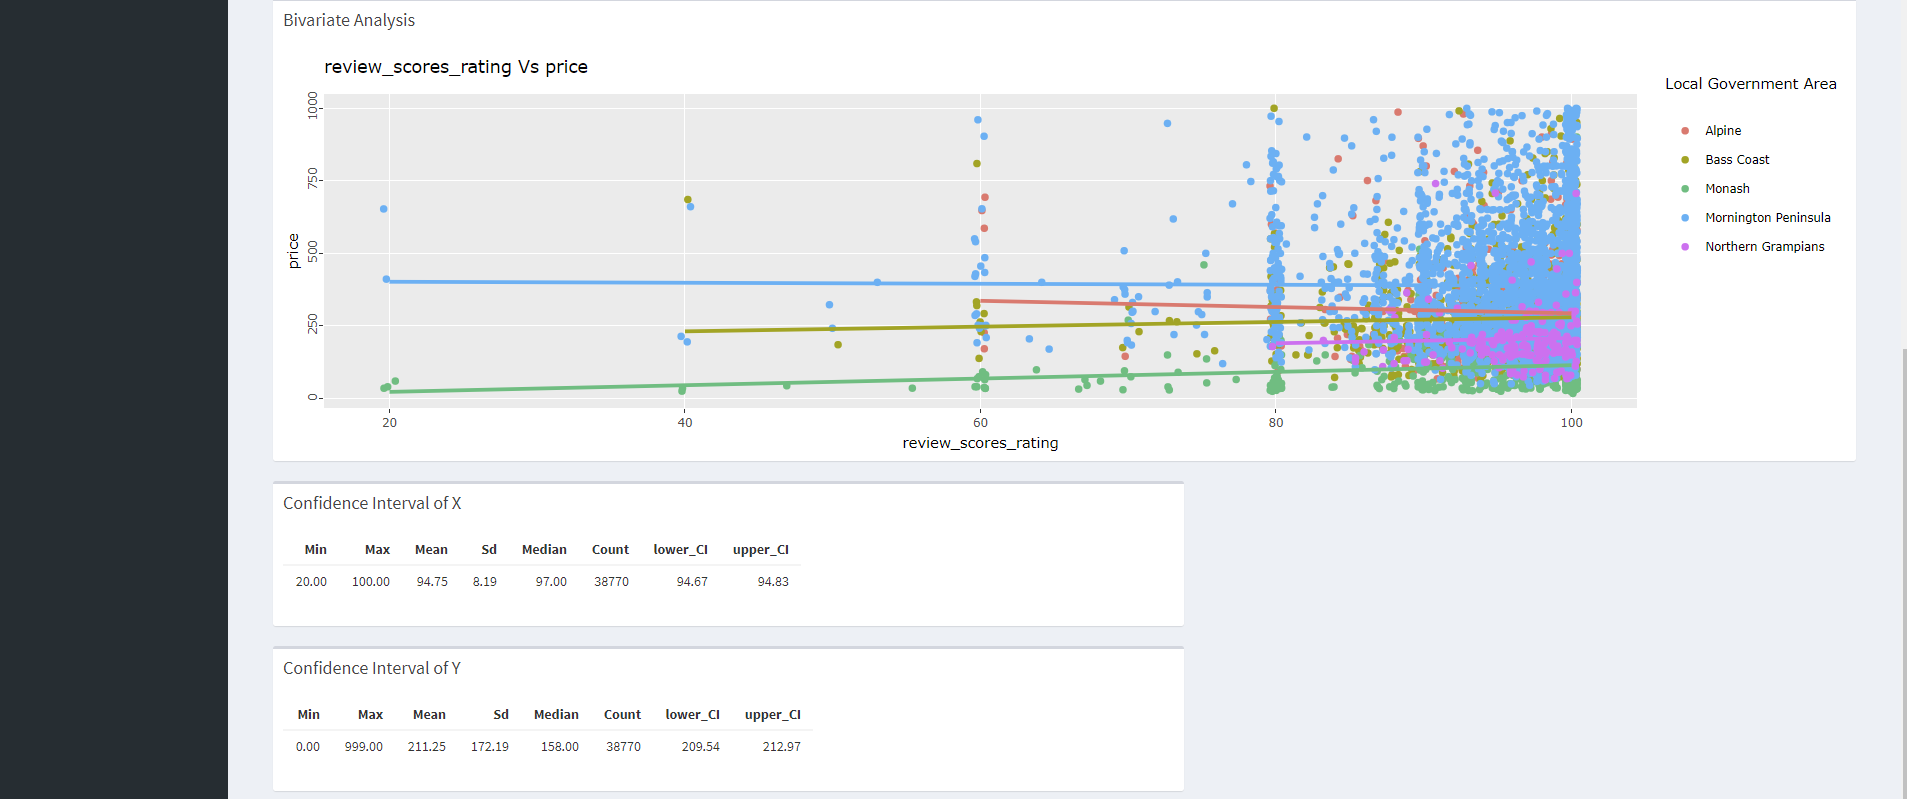
\includegraphics[width=0.6\textwidth,height=\textheight]{images/edabivariate3.png}

The bottom plot is a bivariate plot to explore the relationship between
2 variables.

The two tables below the bivarate plots showcase the confidence interval
of the \emph{``X Variable''} and \emph{``Y Variable:''}.

\hypertarget{correlation-analysis}{%
\subsection{Correlation Analysis}\label{correlation-analysis}}

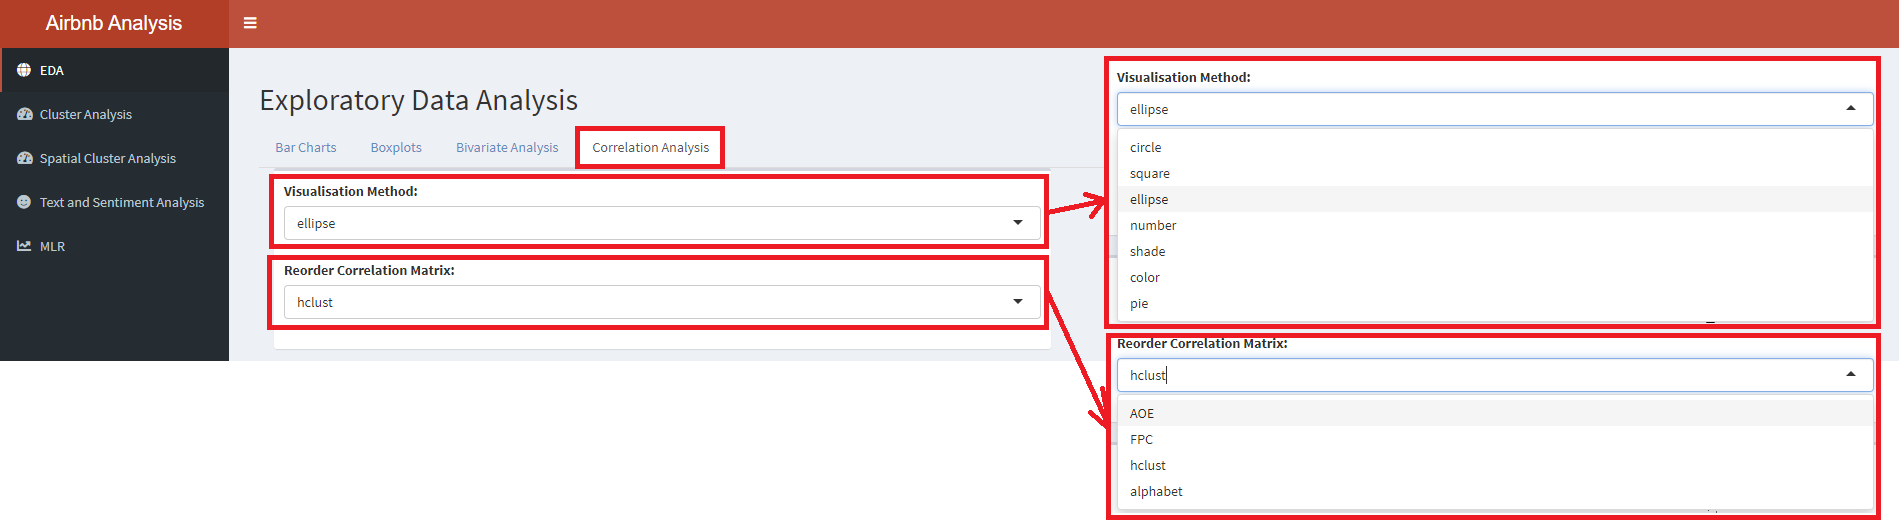
\includegraphics[width=0.6\textwidth,height=\textheight]{images/edacorr.png}

\begin{itemize}
\tightlist
\item
  Click on \emph{``Visualisation Method:''} to view the correlation
  plots in different methods such as \emph{``circle, ellipse and
  number''}.
\item
  Click on \emph{``Reorder Correlation Matrix:''} to view the
  correlation plots in different orders such as \emph{``hclust, alphabet
  and AOE''}.
\end{itemize}

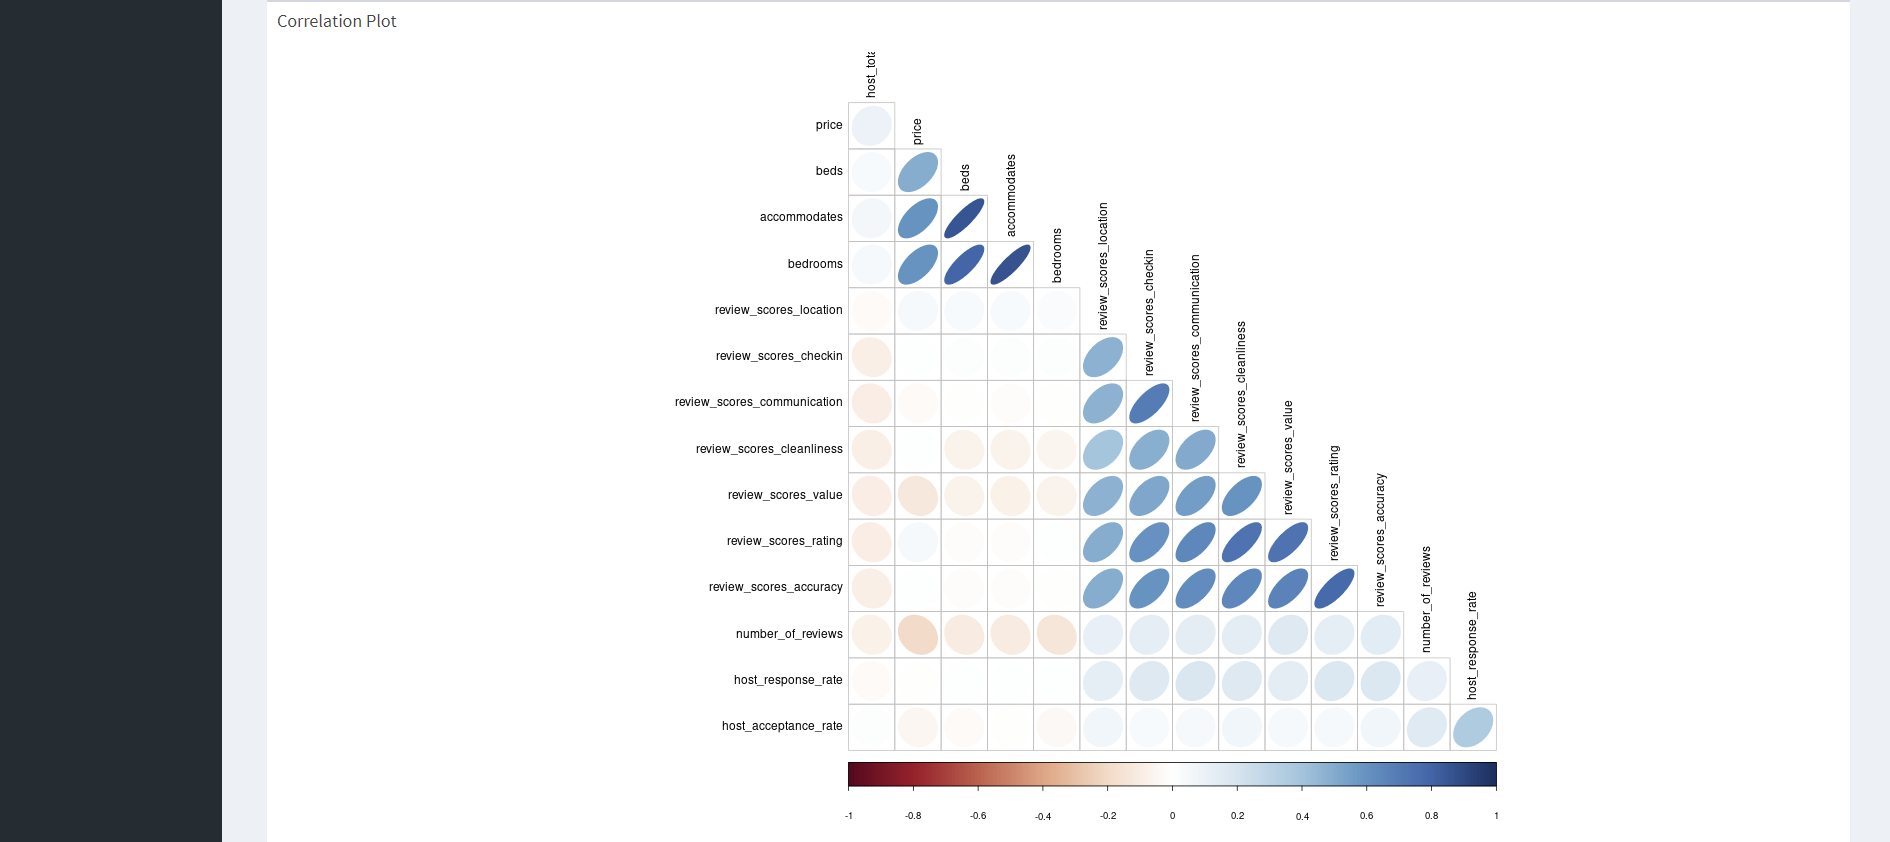
\includegraphics[width=0.6\textwidth,height=\textheight]{images/edacorr2.png}

The plot represents the correlation plot of all the variables in the
Airbnb data set.

\hypertarget{cluster-analysis}{%
\section{Cluster Analysis}\label{cluster-analysis}}

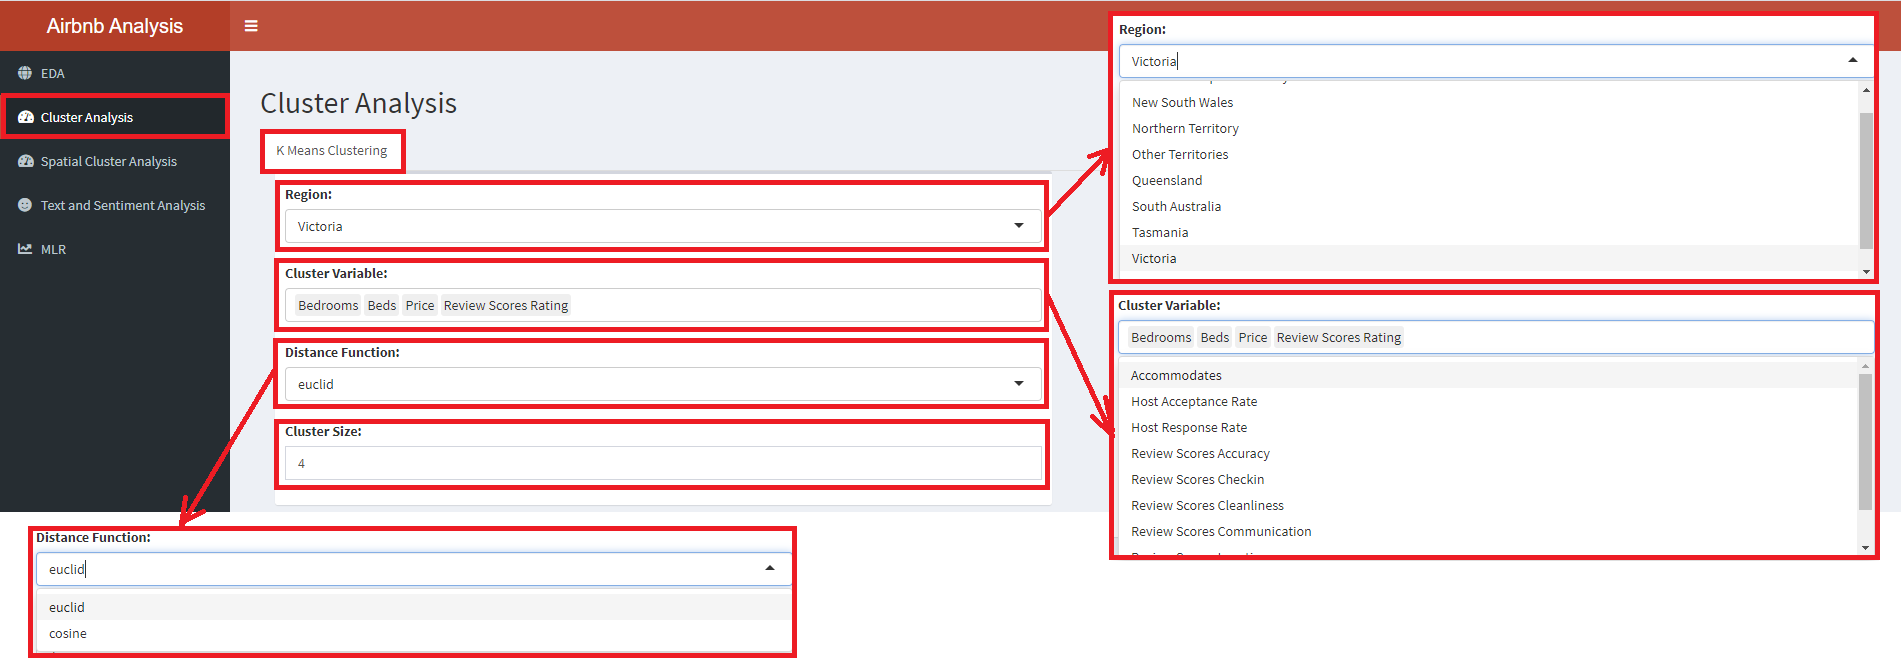
\includegraphics[width=0.6\textwidth,height=\textheight]{images/cluster.png}

\begin{itemize}
\tightlist
\item
  Click on \emph{``Region:''} to explore the different states in
  Australia.
\item
  Click on \emph{``Cluster Variable:''} to explore the different
  variables you would like to cluster. Types of variables are
  \emph{``Price, Bedrooms, Beds, Review Score Ratings''} etc. You are
  also able to click to choose more variables that would be used for
  clustering.
\item
  Click on \emph{``Distance Function:''} to choose between
  \emph{``euclid''} and \emph{``cosine''} distance for the clusters.
\item
  Toggle \emph{``Cluster Size''} between the sizes 2 and 15, to see
  different cluster sizes in the data set.
\end{itemize}

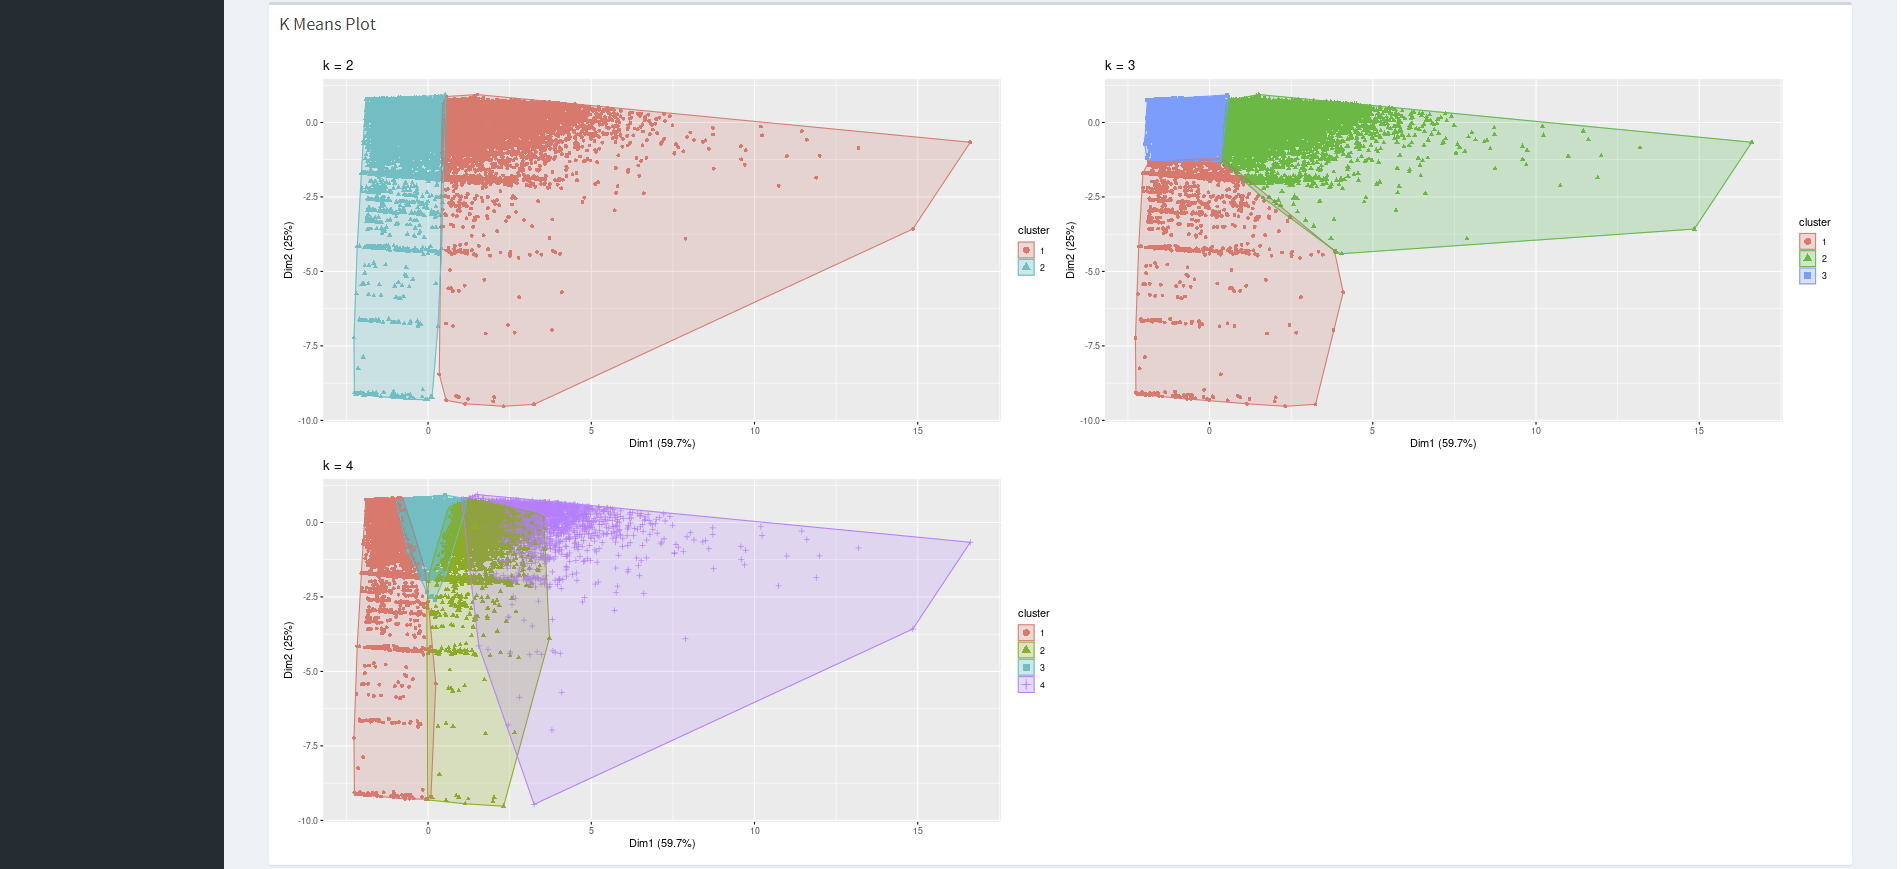
\includegraphics[width=0.6\textwidth,height=\textheight]{images/cluster2.png}

The first plot is the kmeans plot. it showcases the different cluster
sizes.

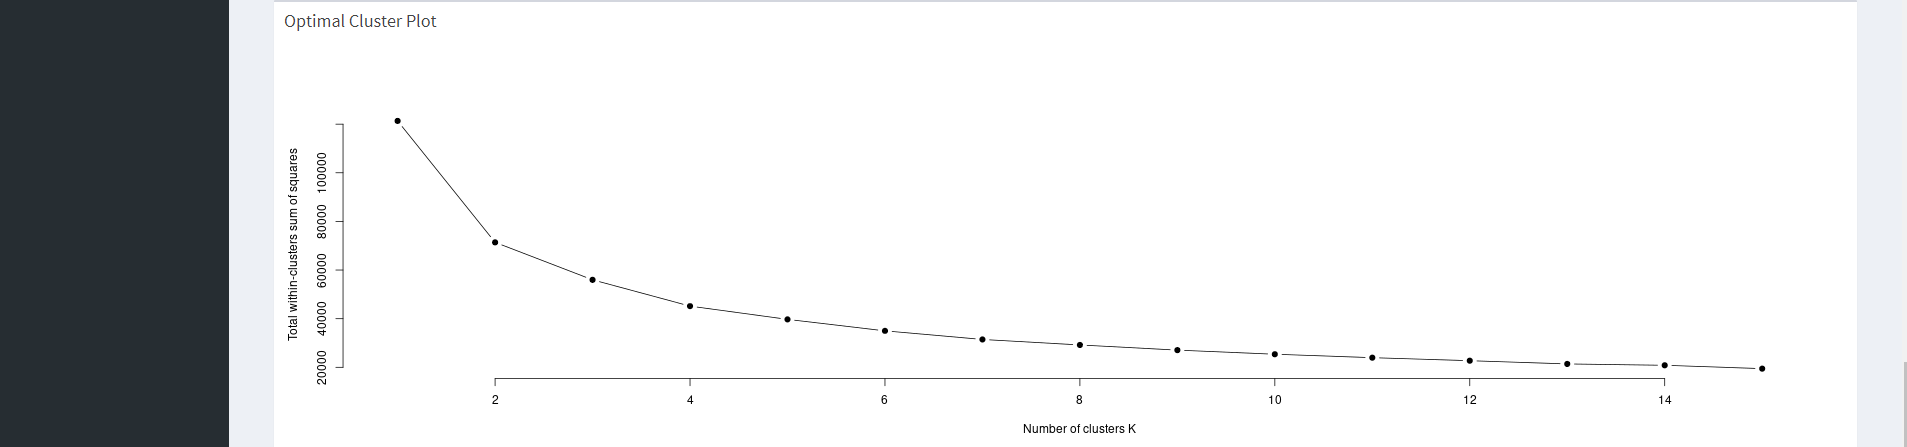
\includegraphics[width=0.6\textwidth,height=\textheight]{images/cluster3.png}

The second plot is an Optimal Cluster Plot, that gives you an indication
the number of clusters that will be best for the data set used.

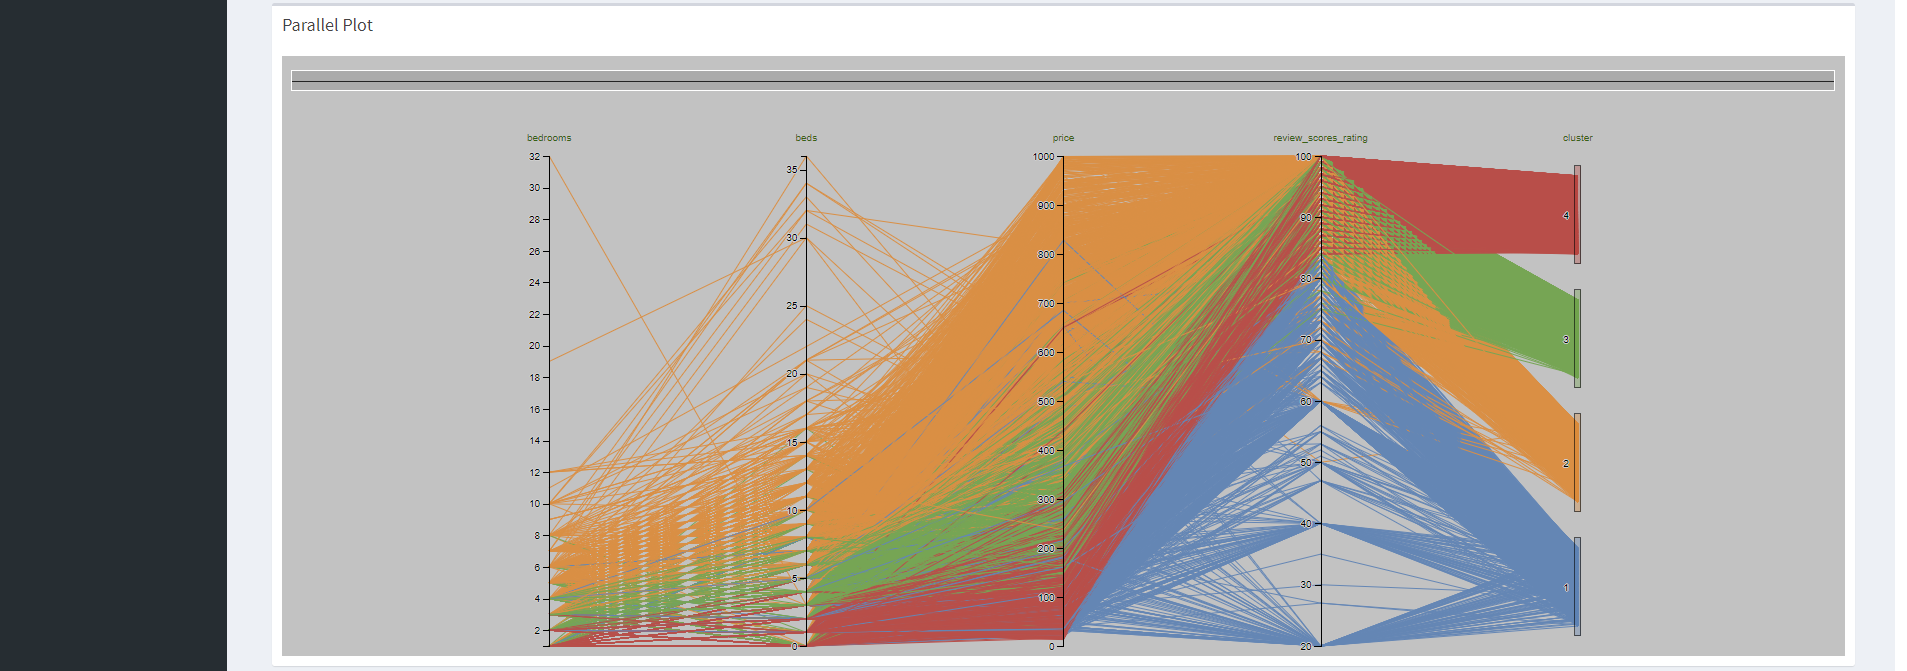
\includegraphics[width=0.6\textwidth,height=\textheight]{images/cluster4.png}

The third plot is a parallel plot that showcases the relationship of the
variables and the clusters. It gives an indication of the
characteristics of the cluster that was formed.

\hypertarget{exploratory-spatial-data-visualization-and-analysis}{%
\section{Exploratory Spatial Data Visualization and
Analysis}\label{exploratory-spatial-data-visualization-and-analysis}}

This tab can be used for exploratory spatial data visualization and
analysis on the Local Government Area (LGA) level for each of the States
of Australia.

Step 1) by clicking on the Spatial Cluster Analysis main left-hand
panel, we enter this tab, with two maps coming into view (Note: it might
take awhile for the viz to load). The left-hand viz provides an overview
of the distribution of either the raw values (default) or clustering
statistics for the LGAs within a selected area (State) of Australia. The
right-hand viz displays the spatial cluster analysis results - showing
areas of high/low clusters, and outliers

Step 2) clicking on the drop down list on the ``Select State:'' tab
allows you to select the state of interest from a list of nine different
states in Australia (\emph{Note: while the visualization allows for user
to select the ``All'' state option, it is highly discouraged as some of
the spatial analyses do not have meaningful interpretations for areas
with considerable missing data - for which at the whole-of-Australia
level, data are more sparsed. When analyzing the data, users are also
advised to conduct due diligence in determining whether the selected
data range of interest has sufficiently satisfied analysis
requirements.})

Step 3) allows you to select the variable of interest from a list of
six..

The resultant maps also allows you to click on the area within each
contiguous boundary to have more information, such as the name of the
LGA, the status (e.g.~(C) is a city, (A) an area, (T) towns, (M)
municipalities, and (S) shire), and the value of the variable of
interest on the first geographical visualization, and the clustering
analysis statistics on the second geo-viz on the right.

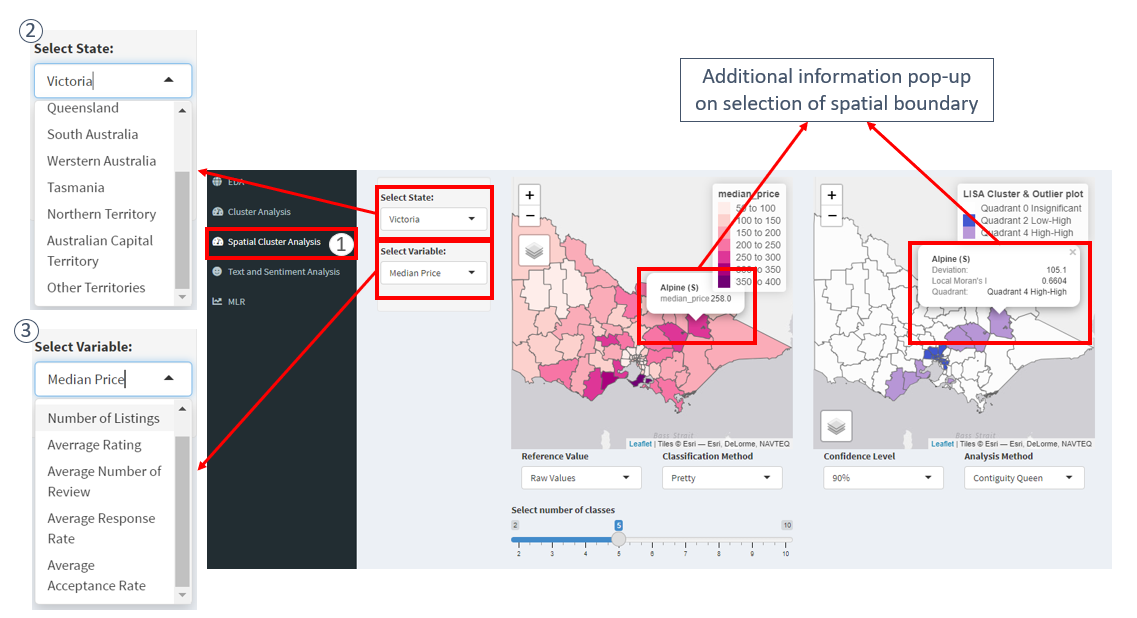
\includegraphics[width=0.6\textwidth,height=\textheight]{images/geospatial1.png}

Step 4) we go on to the options for individual geoviz. For the left-hand
viz, user can first select whether you want the distribution of raw
values displayed, or that of the local indicators of spatial
association's statistics displayed. Note that if the Moran's I's p-value
or the Getis-Ord's G z-scores are selected, selection for other options
(see step 4 and 5 below) will be disabled as these statistical results
are to be interpreted on pre-determined intervals.

Step 5) allows you to select the binning methods - in other words, how
should the values be split up, be it by equal intervals, by natural
breaks (Jenks' and Fisher's), standard deviation bins, etc. A total of
10 options are available under the dropdown.

Step 6) allows user to select the number of intervals to have - i.e.~how
many different classes should the data be split into. User can shift the
slider manually to select the desired class. Note that the selection is
very critical (compulsory) for classification methods such as the K-Mean
selection; practical for methods such as Equal, Pretty, Jenks and
Fisher; but not as useful for methods such as log10 Pretty or even
standard deviation.

Step 7) on the right-hand viz, user can select variables to alter the
clustering parameters. Firstly, the level of confidence - i.e.~how much
confidence do we need to reject the null hypothesis that there are no
spatial clustering/outlier at the areas identified to have such
cluster/outlier.

Step 8) in geospatial analysis, there are also different methods to
select the definition of `neighbor' - this can be selected by changing
the ``Analysis methods:'' panel options. Note that if ``K Nearest
Neighbors'' is selected, an additional slider requesting user to input
the number of nearest neighbors to be considered will appear. Same
thing, if ``Distance'' is selected, a slider to select the distance
radius to be considered neighbor will appear as well.

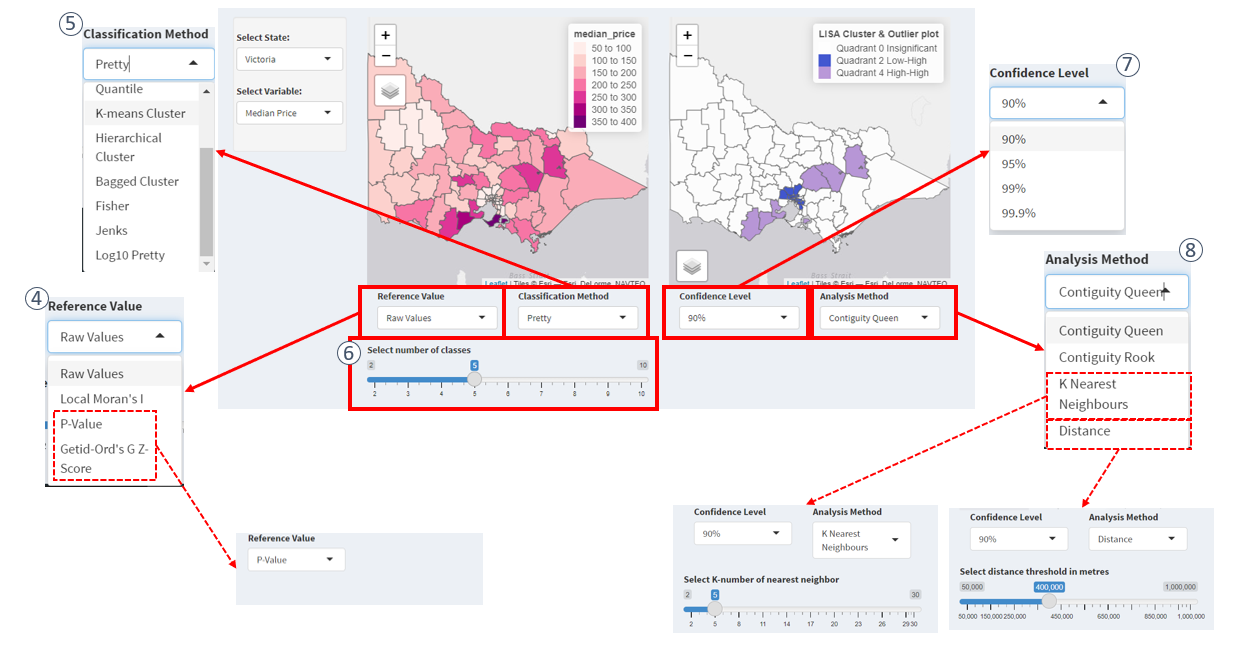
\includegraphics[width=0.6\textwidth,height=\textheight]{images/geospatial2.png}

\hypertarget{sentiment-analysis}{%
\section{Sentiment Analysis}\label{sentiment-analysis}}

The sentiment analysis module of this Shiny app includes two analysis
models: a word cloud and a topic model.

\hypertarget{word-cloud}{%
\subsection{Word Cloud}\label{word-cloud}}

Select the range of review scores rating that you would like to focus
on. By default, all scores are selected.

You can also select which region of Australia you want to focus on.

The word cloud will be generated. The size of the font represents the
relative frequency of the word in the description section of Airbnb
listings that fall in the category of the filter settings above (the
word in the largest font is the most common word).

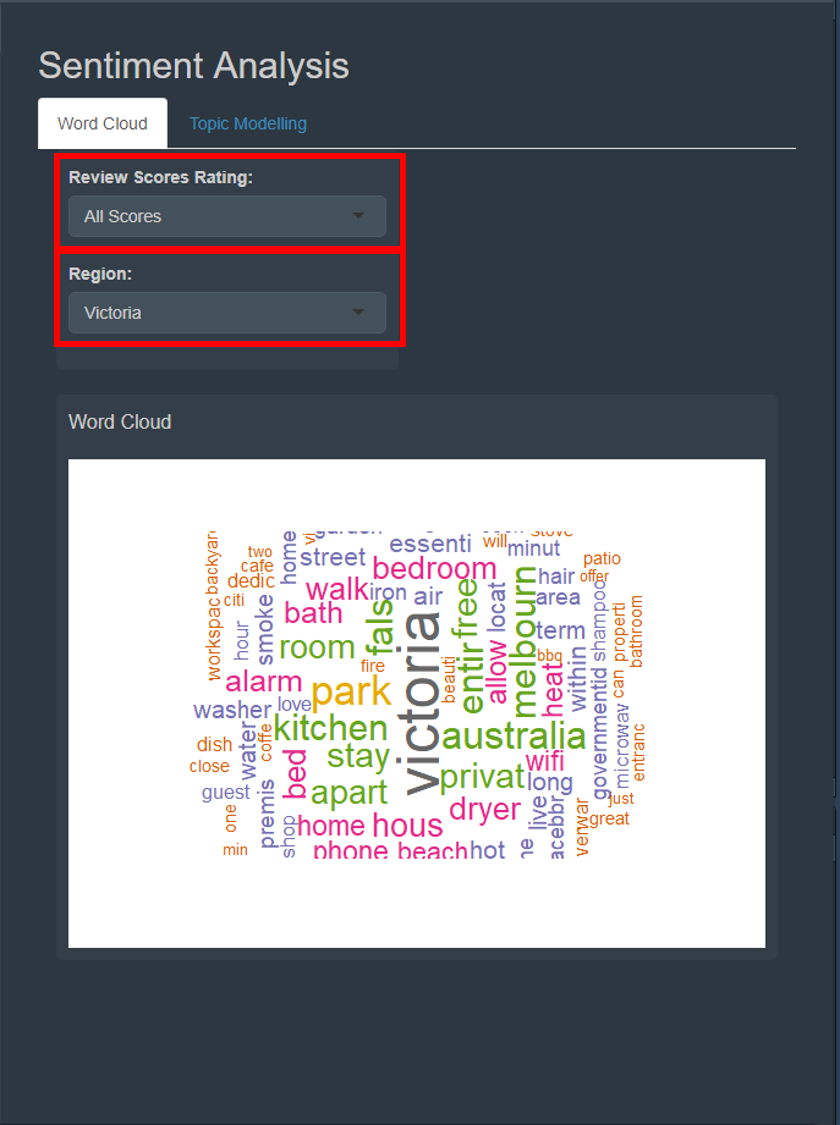
\includegraphics[width=0.6\textwidth,height=\textheight]{images/wordcloud1.png}

\hypertarget{topic-modelling}{%
\subsection{Topic Modelling}\label{topic-modelling}}

Topic modeling is an unsupervised machine learning technique that
detects word and phrase patterns in documents and clusters them into
groups known as topics.

Latent Dirichlet Allocation (LDA) is one common topic modeling
technique. The basic assumption of LDA is that similar topics make use
of similar words (i.e.~distributional hypothesis). The purpose of LDA is
to map the corpus to topics covering a significant number of words in
the documents in the corpus.

LDA assigns topics to arrangements of words for example, the best word
for a topic related to accommodation. This is based on the assumption
that documents are written with a certain arrangement of words and that
those arrangements will determine the topics. LDA assumes that all words
in the document can be assigned a probability of belonging to a topic.
As such, the goal of LDA is to determine the mixture of topics that a
document contains.

Similar to the word cloud, select the range of review scores rating that
you would like to focus on. By default, all scores are selected.

You can also select which region of Australia you want to focus on.

In addition, select how many topics you want to be identified. By
default, the number of topics is 3.

Next, select the number of words you want presented in each topic. The
default number of words is 10.

The LDA topic model will be generated. The bar beside the corresponding
word represents the probability (beta) of that word appearing in that
particular topic. The longer the bar, the higher the probability.

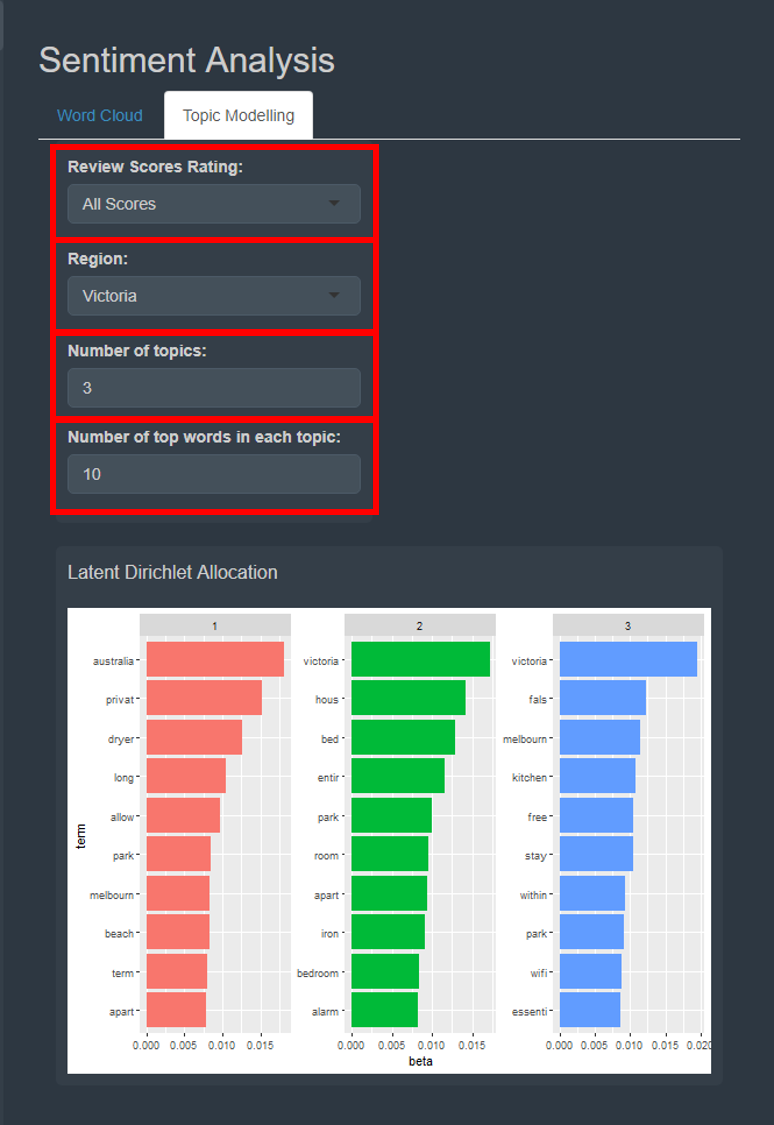
\includegraphics[width=0.6\textwidth,height=\textheight]{images/topicmodel1.png}

\hypertarget{multiple-linear-regression}{%
\section{Multiple Linear Regression}\label{multiple-linear-regression}}

\hypertarget{regression-for-price}{%
\subsection{Regression for Price}\label{regression-for-price}}

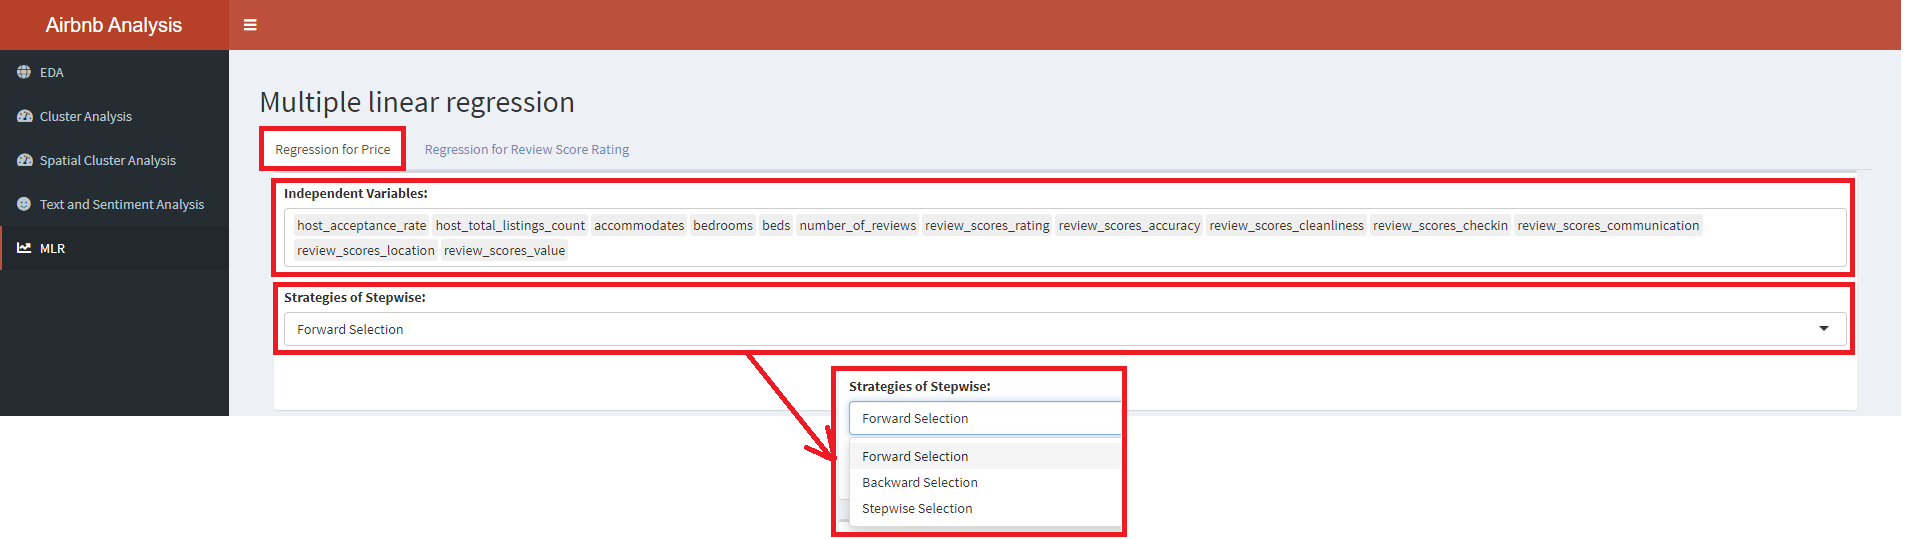
\includegraphics[width=0.6\textwidth,height=\textheight]{images/mlr.png}

\begin{itemize}
\tightlist
\item
  Click on \emph{``Independent Variables:''} to choose the multiple
  variables that you would like to apply in the Multiple Linear
  Regression (MLR). The choices of variables could be influenced through
  the correlation plot found in the EDA. It is better to choose
  variables with low correlation with each other.
\item
  Click on \emph{``Strategies of Stepwise:''} to choose whether the MLR
  will move in a \emph{``Forward'', ``Backward'',} or
  \emph{``Stepwise''} direction.
\end{itemize}

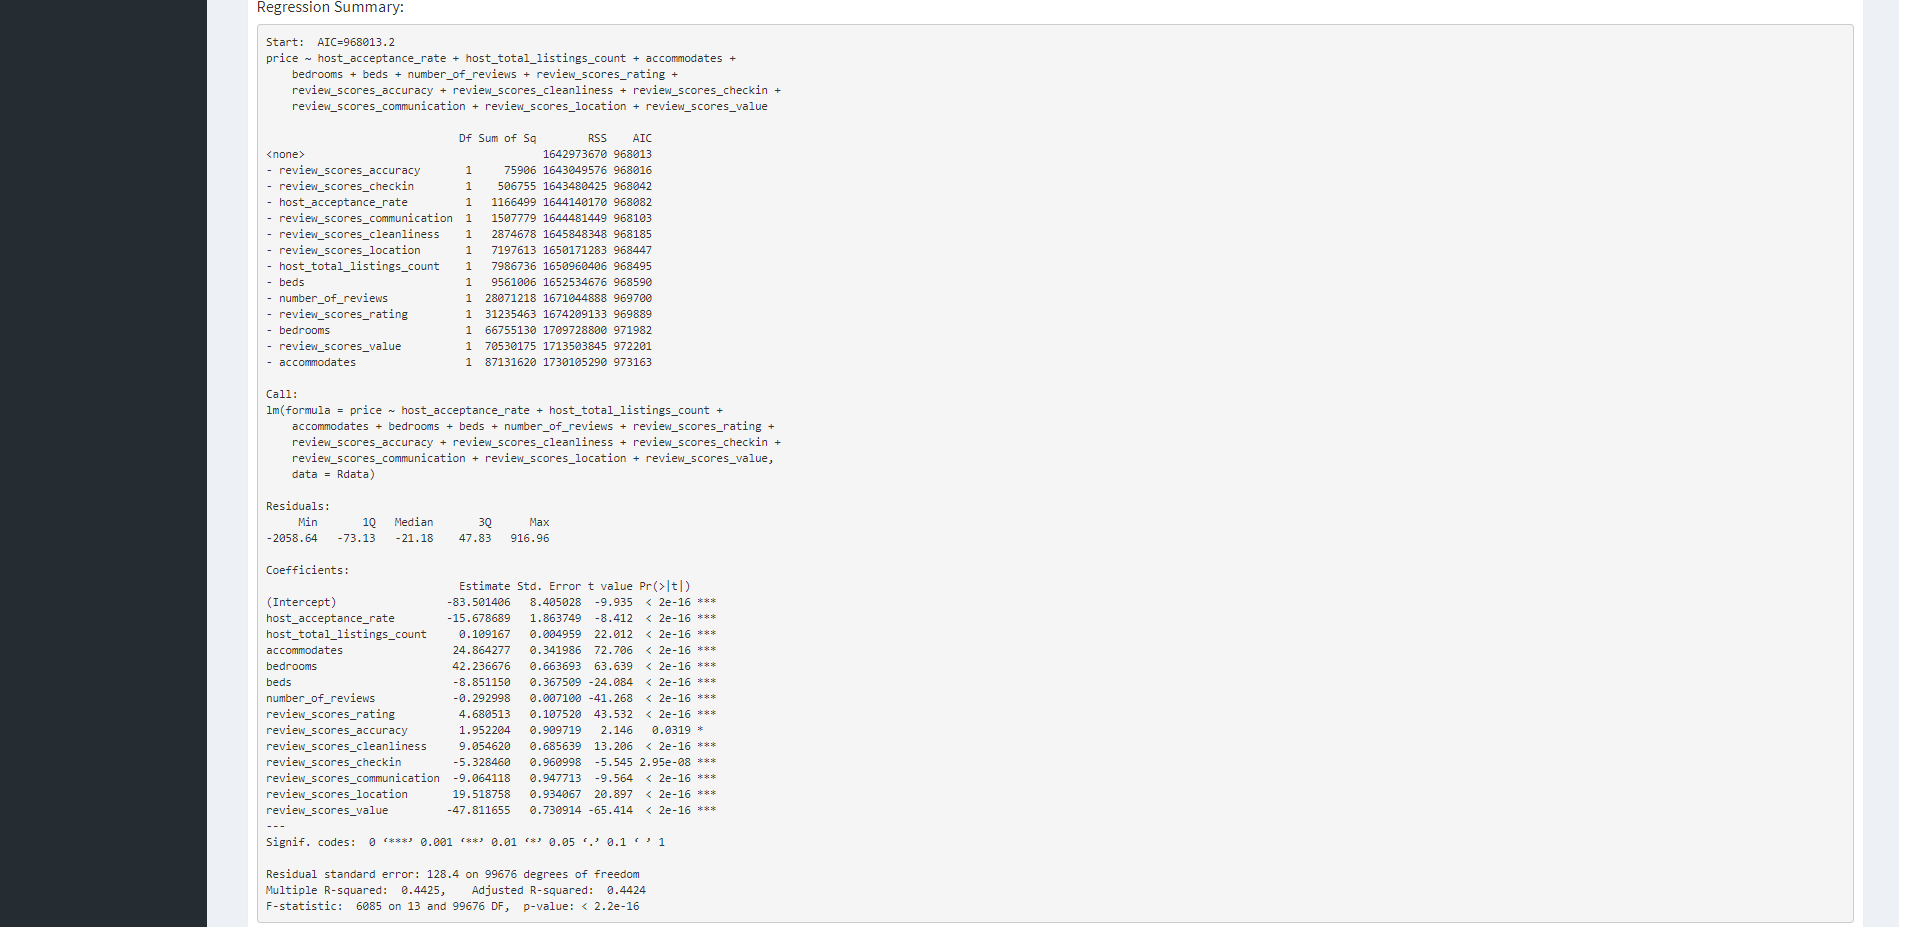
\includegraphics[width=0.6\textwidth,height=\textheight]{images/mlr2.png}

The \emph{``Regression Summary''} showcases the MLR calculation and
gives us an indication of the significance of each variable in the
regression with respect to \emph{``Price''}.

\hypertarget{regression-for-review-score-ratings}{%
\subsection{Regression for Review Score
Ratings}\label{regression-for-review-score-ratings}}

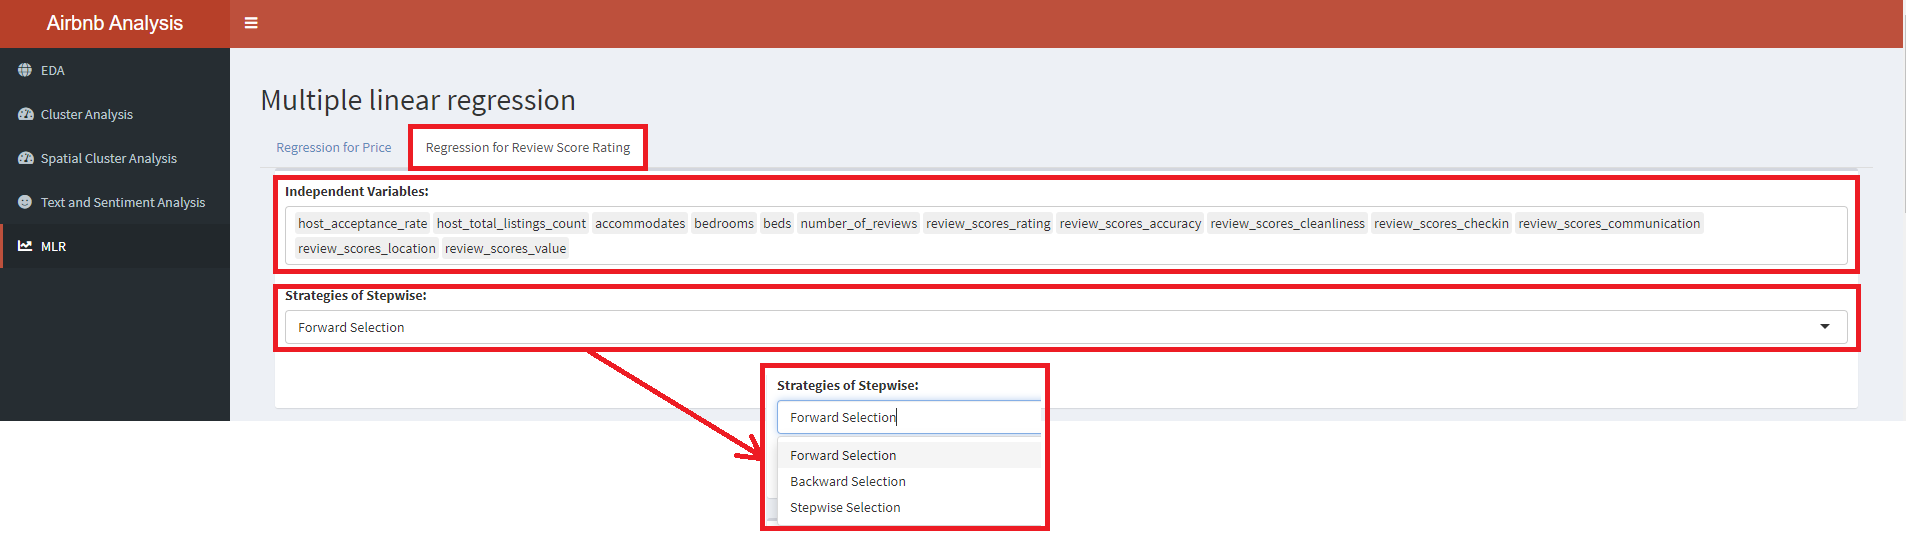
\includegraphics[width=0.6\textwidth,height=\textheight]{images/mlr3.png}

\begin{itemize}
\tightlist
\item
  Click on \emph{``Independent Variables:''} to choose the multiple
  variables that you would like to apply in the Multiple Linear
  Regression (MLR). The choices of variables could be influenced through
  the correlation plot found in the EDA. It is better to choose
  variables with low correlation with each other.
\item
  Click on \emph{``Strategies of Stepwise:''} to choose whether the MLR
  will move in a \emph{``Forward'', ``Backward'',} or
  \emph{``Stepwise''} direction.
\end{itemize}

The \emph{``Regression Summary''} showcases the MLR calculation and
gives us an indication of the significance of each variable in the
regression with respect to \emph{``Review Score Ratings''}.

\end{document}
